\documentclass{beamer}
\usepackage[utf8]{inputenc}
\usepackage[english]{babel}
\usepackage{helvet}
\usepackage[T1]{fontenc}
\usepackage{textcomp}
\usepackage[inline]{asymptote}
\usepackage{slide_helper}
\usepackage{multirow}
\usepackage{tikz}
\usepackage{subfigure}
\usetikzlibrary{shapes.geometric, arrows}
\usepackage{pgfplots}
\pgfplotsset{compat=1.5} 
\usepgfplotslibrary{statistics}
\usetikzlibrary{external}
\tikzexternalize%

\title[MA205 - Section 3.1]{Defining Probability}

\DeclareSymbolFont{extraup}{U}{zavm}{m}{n}
\DeclareMathSymbol{\varheart}{\mathalpha}{extraup}{86}
\DeclareMathSymbol{\vardiamond}{\mathalpha}{extraup}{87}
\DeclareMathSymbol{\varclub}{\mathalpha}{extraup}{84} 
\DeclareMathSymbol{\varspade}{\mathalpha}{extraup}{85}

\newcommand{\suitheart}[1][]{{\color{red}\text{#1}\varheart}}
\newcommand{\suitspade}[1][]{{\color{black}\text{#1}\spadesuit}}
\newcommand{\suitdiamond}[1][]{{\color{red}\text{#1}\vardiamond}}
\newcommand{\suitclub}[1][]{{\color{black}\text{#1}\varclub}}
\newcommand{\card}[2]{{#1{\color{black}\text{#2}}}}

\newcommand{\prob}[1]{P\left(#1\right)}
\newcommand{\condprob}[2]{\prob{#1~\middle|~#2}}
\newcommand{\comb}[2]{_{#1}C_{#2}}

\begin{document}
\begin{frame}
\titlepage
\end{frame}

\begin{frame}
\begin{definition}
The result of \textbf{random process} is called an \textbf{outcome}.
\end{definition}\pause

\begin{note}
A \textbf{die}, the singular of \textbf{dice}, is a cube with six sides numbered 1 to 6.
\end{note}\pause

\begin{example}
Assume we roll a die and get a 1.

\vspace{1mm}
\question{What is the random process?}\pause
\answer{Rolling the die.}\pause

\vspace{1mm}
\question{What is the outcome?}\pause
\answer{The 1 that was rolled.}\pause

\vspace{1mm}
\question{What is the chance of rolling a 1 on this die?}\pause
\answer{If the dice is fair, each side has the same chance of being rolled. So a 1 has a one-in-six chance, equivalently $\dfrac{1}{6}$.}
\end{example}
\end{frame}

\begin{frame}
\begin{definition}
A \textbf{probability} of an outcome is the proportion of times the outcome would occur if we observed the random process an infinite number of times.
\end{definition}\pause

\begin{note}
\begin{equation*}
\prob{X}=\dfrac{\text{Number of outcomes corresponding to $X$}}{\text{Total number of outcomes}}
\end{equation*}
\end{note}\pause

\begin{example}
\question{What is the probability of rolling a 1 or 2 on a die?}\pause
\answer{There are two outcomes, a 1 or a 2, and six faces on a die.
\begin{equation*}
\prob{\text{roll}~1~\text{or}~2} = \dfrac{2}{6} = \dfrac{1}{3}
\end{equation*}}
\end{example}
\end{frame}

\begin{frame}
\begin{note}
A standard deck of 52 playing cards consists of four \textbf{suits} in two colors: 
Hearts $\suitheart$, Spades $\suitspade$, Diamonds $\suitdiamond$, and Clubs $\suitclub$

\vspace{2mm}
Each suit contains 13 cards, each of a different \textbf{rank}: \\
2 through 10, Jack, Queen, King, and Ace

\vspace{2mm}
The Jack, Queen, and King cards are called \textbf{face cards}.

\vspace{2mm}
The Jack, Queen, King, and Ace cards are called \textbf{honour cards}.

\vspace{2mm}
The cards numbered 2 to 10 are called \textbf{numerals}.
\vspace{-1mm}
\begin{equation*}
\begin{array}{ccccccccccccc}
\card{\suitclub}{2} & \card{\suitclub}{3} & \card{\suitclub}{4} & \card{\suitclub}{5} & \card{\suitclub}{6} & \card{\suitclub}{7} & \card{\suitclub}{8} & \card{\suitclub}{9} & \card{\suitclub}{10} & \card{\suitclub}{J} & \card{\suitclub}{Q} & \card{\suitclub}{K} &\card{\suitclub}{A} \\
\card{\suitdiamond}{2} & \card{\suitdiamond}{3} & \card{\suitdiamond}{4} & \card{\suitdiamond}{5} & \card{\suitdiamond}{6} & \card{\suitdiamond}{7} & \card{\suitdiamond}{8} & \card{\suitdiamond}{9} & \card{\suitdiamond}{10} & \card{\suitdiamond}{J} & \card{\suitdiamond}{Q} & \card{\suitdiamond}{K} &\card{\suitdiamond}{A} \\
\card{\suitheart}{2} & \card{\suitheart}{3} & \card{\suitheart}{4} & \card{\suitheart}{5} & \card{\suitheart}{6} & \card{\suitheart}{7} & \card{\suitheart}{8} & \card{\suitheart}{9} & \card{\suitheart}{10} & \card{\suitheart}{J} & \card{\suitheart}{Q} & \card{\suitheart}{K} &\card{\suitheart}{A} \\
\card{\suitspade}{2} & \card{\suitspade}{3} & \card{\suitspade}{4} & \card{\suitspade}{5} & \card{\suitspade}{6} & \card{\suitspade}{7} & \card{\suitspade}{8} & \card{\suitspade}{9} & \card{\suitspade}{10} & \card{\suitspade}{J} & \card{\suitspade}{Q} & \card{\suitspade}{K} &\card{\suitspade}{A}
\end{array}
\end{equation*}
\end{note}
\end{frame}

\begin{frame}
\begin{example}
\question{What is the probability of drawing a single card from a deck and getting an Ace?}\pause
\answer{There are four aces in a deck of 52 cards. Which gives the probability
\begin{equation*}
\prob{\text{Ace}}=\dfrac{4}{52}=\dfrac{1}{13}= 0.0769=7.67\%
\end{equation*}}
\vspace{-4mm}
\end{example}\pause


\begin{example}
\question{What is the probability of rolling a 1, 2, 3, 4, 5, or 6 on a die?}\pause
\answer{Every side of the die is listed, so
\begin{equation*}
\prob{\text{roll}~1~\text{or}~2~\text{or}~3~\text{or}~4~\text{or}~5~\text{or}~6} = \dfrac{6}{6} = 1 = 100\%
\end{equation*}}
\vspace{-4mm}
\end{example}\pause

\begin{definition}
An outcome with a probability of 1 is called \textbf{certain}.
\end{definition}
\end{frame}

\begin{frame}
\begin{example}
\question{If a year is selected at random, what is the probability that Thanksgiving Day (in the United States) will be on a Wednesday?}\pause
\answer{In the United States, Thanksgiving Day always falls on the fourth Thursday in November. \pause

\vspace{1mm}
This means it is impossible for Thanksgiving Day to fall on a Wednesday.
\begin{equation*}
\begin{aligned}
\prob{\text{Thanksgiving on a Wednesday}}&=0=0\%\\
\prob{\text{Thanksgiving on a Thursday}}&=1=100\%
\end{aligned}
\end{equation*}}
\end{example}\pause

\begin{definition}
An outcome with a probability of 0 is called \textbf{impossible}.
\end{definition}\pause

\begin{note}
Probabilities are always between 0 and 1.
\end{note}
\end{frame}

\begin{frame}
\begin{example}
The probability of rolling a 1 on a die is $p=1/6\approx0.167$, but if we roll six dice, we may get no 1's or multiple 1's.\pause

\vspace{1mm}
Let $\hat{p}_n$ be the proportion of number of 1's rolled after $n$ rolls.

\begin{center}
\begin{tikzpicture}
%\pgfkeys{/pgf/number format/.cd,
%fixed,
%precision=999,
%set thousands separator={,},
%1000 sep in fractionals=true,
%}
\begin{semilogxaxis}[
clip mode=individual,
clip marker paths=true,
width=11.5cm,
height=5cm,
xlabel={$n$ (number of rolls)},
ylabel={$\hat{p}_n$},
ylabel style={rotate=-90},
grid=major,
minor tick style={draw=none},
xtick={1, 10, 100, 1000, 10000, 100000},
xticklabels={1,10,100,{1,000},{10,000},{100,000}},
]
\draw[red!90, dashed] (-1.1, 166) -- (12.6,166); % super hack-y, but I couldn't figure how how to get a wide enough line in axis cs
\addplot [blue!85] table [y=pn, x=n, col sep=comma] {diceroll.csv};
\end{semilogxaxis}
\end{tikzpicture}
\end{center}\pause
\end{example}
\begin{note}
It is not a coincidence that $\hat{p}_n$ get closer to $p$ as $n$ increases.
\end{note}
\end{frame}

\begin{frame}
\begin{block}{Law of Large Numbers}
As more observations are collected, the proportion $\hat{p}_n$ of occurrences with a particular outcome converges to the probability $p$ of that outcome.
\end{block}\pause

\begin{block}{Cautions}
\begin{itemize}
\item The law of large numbers applies to behavior over a large number of trails, and it does not apply to any one individual outcome.\pause
\begin{itemize}
\item Gamblers sometimes foolishly loose large sums of money by incorrectly thinking that a string of losses increases the chances of a win on the next bet, or that a string of wins is likely to continue.
\end{itemize}\pause
\item If we know nothing about the likelihood of different possible outcomes, we should not assume that they are equally likely.\pause
\begin{itemize}
\item You should not think that the probability of passing the next exam is $\tfrac{1}{2}$, or 0.5. The actual probability depends on factors such as the amount of preparation and the difficulty of the exam.
\end{itemize}
\end{itemize}
\end{block}
\end{frame}

\begin{frame}
\begin{definition}
Outcomes $A$ and $B$ are \textbf{disjoint} (or \textbf{mutually exclusive}) if they cannot occur at the same time.
\end{definition}\pause

\begin{example}
\question{Are the outcomes \textquote{roll a 1} and \textquote{roll a 2} disjoint?}\pause
\answer{Yes, it is impossible to roll two different numbers at the same time.}
\end{example}\pause

\begin{example}
\question{Are the outcomes \textquote{roll a 1} and \textquote{roll an odd number} disjoint?}\pause
\answer{No, 1 is an odd number.}
\end{example}\pause

\begin{example}
\question{Are the outcomes \textquote{draw an ace} and \textquote{draw a diamond} disjoint?}\pause
\answer{No, the $\card{\suitdiamond}{A}$ is both an ace and a diamond.}
\end{example}
\end{frame}

\begin{frame}
\begin{block}{Addition Rule of Disjoint Outcomes}
If $A_1$ and $A_2$ represent two disjoint outcomes, then the probability that one of them occurs is given by:
\begin{equation*}
\prob{A_1~\text{or}~A_2} = \prob{A_1} + \prob{A_2}
\end{equation*}
\end{block}\pause

\begin{example}
The probability of rolling a 1 or rolling a 2 on a die can be calculated two ways:\pause

\vspace{1mm}
\textbf{Directly:} There are two outcomes that are either a 1 or a 2, so the probability is:
\begin{equation*}
\prob{\text{roll a 1 or roll a 2}} = \dfrac{2}{6} = \dfrac{1}{3}
\end{equation*}\pause

\vspace{-4mm}
\textbf{Addition Rule}: Rolling a 1 and rolling a 2 are disjoint, so:
\begin{equation*}
\begin{aligned}
\prob{\text{roll a 1 or roll a 2}} &= \prob{\text{roll a 1}} + \prob{\text{roll a 2}} \\\pause
&= \dfrac{1}{6} + \dfrac{1}{6}
= \dfrac{1+1}{6} 
= \dfrac{2}{6} 
= \dfrac{1}{3}
\end{aligned}
\end{equation*}
\end{example}
\end{frame}

\begin{frame}
\begin{example}
Let's calculate the probability of rolling a 1, 2, or 3.\pause
\begin{equation*}
\begin{aligned}
\prob{\text{roll a 1 or roll a 2 or roll a 3}} &= \prob{\text{roll a 1}} + \prob{\text{roll a 2}} + \prob{\text{roll a 3}} \\\pause
&= \dfrac{1}{6} + \dfrac{1}{6} + \dfrac{1}{6}\\\pause
&=\dfrac{3}{6}
=\dfrac{1}{2}
\end{aligned}
\end{equation*}
\end{example}\pause

\begin{example}
Let's calculate the probability of rolling a 1, 2, 3 or 4.\pause
\begin{equation*}
\begin{aligned}
\prob{\text{roll a 1 or 2 or 3 or 4}} &= \prob{\text{1}} + \prob{\text{2}} + \prob{\text{3}} + \prob{\text{4}}  \\\pause
&= \dfrac{1}{6} + \dfrac{1}{6} + \dfrac{1}{6}+ \dfrac{1}{6}\\\pause
&=\dfrac{4}{6}
=\dfrac{2}{3}
\end{aligned}
\end{equation*}
\end{example}
\end{frame}

\begin{frame}
\begin{definition}
A \textbf{event} is a collection of outcomes.
\end{definition}\pause

\begin{note}
If two events have no elements in common, they are disjoint.
\end{note}\pause

\begin{example}
Consider the following events.
\begin{center}
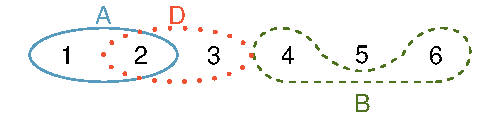
\includegraphics{disjointSets.pdf}
\end{center}\pause

\question{Are A and B disjoint?}\pause
\answersingleline{Yes.}\pause

\vspace{1mm}
\question{Are A and D disjoint?}\pause
\answersingleline{No, 2 is in both.}\pause

\vspace{1mm}
\question{Are B and D disjoint?}\pause
\answersingleline{Yes.}
\end{example}
\end{frame}

\begin{frame}
\begin{example}
Suppose we flip a fair coin and roll a fair die. 

\vspace{2mm}
The list of all possible outcomes is:
\begin{center}
\text{H1}, \text{H2}, \text{H3}, \text{H4}, \text{H5}, \text{H6}, \text{T1}, \text{T2}, \text{T3}, \text{T4}, \text{T5}, \text{T6}
\end{center}\pause

We want to calculate the probability of getting a head or a six.\pause

\vspace{2mm} 
The relevant outcomes are: H1, H2, H3, H4, H5, H6, T6. 

\vspace{2mm}
Meaning that $\prob{\text{H or 6}} = \tfrac{7}{12}$.\pause

\vspace{2mm}
Notice that $\tfrac{6}{12}=\tfrac{1}{2}$ of the outcomes have heads and $\tfrac{2}{12}=\tfrac{1}{6}$ have a six. \pause

\vspace{2mm}
But, $\tfrac{1}{2}+\tfrac{1}{6}=\frac{8}{12}$, is wrong because we have double counted H6. \pause

\vspace{2mm}
The correct probability is:

\vspace{-3mm}
\begin{equation*}
\prob{\text{H or 6}} = \prob{\text{H}}+\prob{6}-\prob{\text{H and 6}}\pause = \tfrac{1}{2}+\tfrac{1}{6}-\tfrac{1}{12}\pause =\tfrac{7}{12}
\end{equation*}
\vspace{-4mm}
\end{example}
\end{frame}

\begin{frame}
\begin{example}
Let us consider the events \textquote{draw a diamond} and \textquote{draw a face card}.\pause

\vspace{1mm}
These outcomes are not disjoint, since three cards are both:

\begin{center}
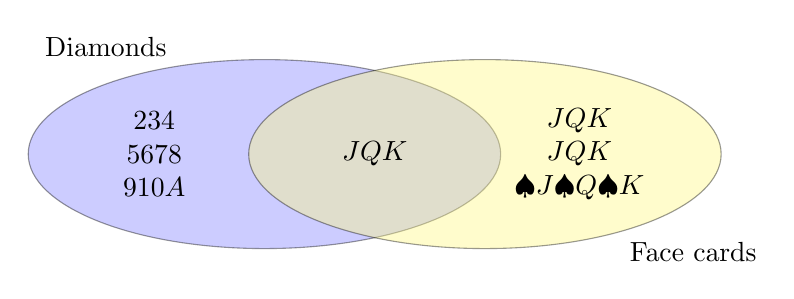
\begin{tikzpicture}[every text node part/.style={align=center}]
% Set A
\node [draw,
    ellipse,
    fill=blue!50,
    opacity=0.4,
    label={135:Diamonds},
    minimum height = 2.4cm,
    minimum width = 6cm] (A) at (0,0){};
 
% Set B
\node [draw,
    ellipse,
    fill=yellow!50,
    opacity=0.4,
    label={-30:Face cards},
    minimum height = 2.4cm,
    minimum width = 6cm] (B) at (2.8,0){};
 
% Set intersection label
\node at (1.4,0) {$\card{\suitdiamond}{J}\card{\suitdiamond}{Q}\card{\suitdiamond}{K}$};
\node at (-1.4,0) {$\card{\suitdiamond}{2}\card{\suitdiamond}{3}\card{\suitdiamond}{4}$ \\ $\card{\suitdiamond}{5}\card{\suitdiamond}{6}\card{\suitdiamond}{7}\card{\suitdiamond}{8}$ \\ $\card{\suitdiamond}{9}\card{\suitdiamond}{10}\card{\suitdiamond}{A}$};
\node at (4,0) {$\card{\suitclub}{J}\card{\suitclub}{Q}\card{\suitclub}{K}$ \\ $\card{\suitheart}{J}\card{\suitheart}{Q}\card{\suitheart}{K}$ \\ $\card{\suitspade}{J}\card{\suitspade}{Q}\card{\suitspade}{K}$};
\end{tikzpicture}
\end{center}\pause
The Addition Rule for Disjoint Outcomes would count $\card{\suitdiamond}{J}\card{\suitdiamond}{Q}\card{\suitdiamond}{K}$ twice!\pause

\vspace{-1mm}
\begin{equation*}
\begin{aligned}
\prob{\suitdiamond~\text{and}~\text{face}} &= \prob{\suitdiamond} + \prob{\text{face}} - \prob{\suitdiamond~\text{and}~\text{face}} \\\pause
&= \hspace{2mm}\dfrac{13}{52}\pause \hspace{2.5mm}+\hspace{3mm} \dfrac{12}{52}\pause \hspace{5.5mm}- \hspace{3mm}\dfrac{3}{52} \\\pause
&= \hspace{2mm}\dfrac{22}{52} = \dfrac{11}{26}
\end{aligned}
\end{equation*}
\end{example}
\end{frame}

\begin{frame}
\begin{block}{General Addition Rule}
If $A$ and $B$ are any two events, disjoint or not, then the probability that at least one of them will occur is:
\begin{equation*}
\prob{A~\text{or}~B} = \prob{A}+\prob{B}-\prob{A~\text{and}~B}
\end{equation*}
\end{block}\pause

\begin{note}
In statistics, when we write \textquote{or} what we mean is \textquote{and/or}, unless we explicitly say otherwise.

\vspace{1mm}
In other words, \textquote{$A$ or $B$} occurring means $A$, $B$, or both $A$ and $B$ occur.
\end{note}\pause

\begin{note}
If $A$ and $B$ are disjoint this means $\prob{A~\text{and}~B}=0$, and so we get the Addition Rule for Disjoint Outcomes:

\vspace{-2mm}
\begin{equation*}
\begin{aligned}
\prob{A~\text{or}~B} &= \prob{A}+\prob{B}-\prob{A~\text{and}~B} \\
&= \prob{A}+\prob{B} - 0 \\
&= \prob{A}+\prob{B}
\end{aligned}
\end{equation*}
\end{note}
\end{frame}

\begin{frame}
\begin{example}
Suppose we draw one card from a standard deck. Let us find the probability that we get a Queen or a King.\pause

\vspace{2mm}
There are 4 Queens and 4 Kings in the deck, hence eight outcomes out of 52 possible outcomes. So, the probability is
\begin{equation*}
\prob{\text{Q or K}} = \dfrac{8}{52}
\end{equation*}\pause

Since there are no cards that are both Kings and Queens, we have
\begin{equation*}
\prob{\text{Q or K}} = \prob{\text{Q}} + \prob{K} - \prob{\text{Q and K}} = \dfrac{4}{52}+\dfrac{4}{52}-\dfrac{0}{52} = \dfrac{8}{52}
\end{equation*}
\end{example}
\end{frame}
\end{document}
